\chapter{Entwurfsmuster}
\paragraph{Beobachter}
Ein im Quellcode des Programms identifiziertes Entwurfsmuster ist das des Beobachters. Dieses findet sich in der \href{https://github.com/EinToni/Wortfinder/blob/main/Wortfinder/GameTimer.cs}{\textit{GameTimer}} und \href{https://github.com/EinToni/Wortfinder/blob/main/Wortfinder/GameManager.cs}{\textit{GameManager}} Klasse wieder. Der \textit{GameManager} registriert dabei zwei Callback-Funktionen beim \textit{GameTimer}. Nachdem der Timer gestartet wurde, wird die eine Funktion jede Sekunde, also jeden Tick des Timers, aufgerufen und die andere, sobald der Timer 0 erreicht. Der \textit{GameTimer} ist daher das Subjekt und der \textit{GameManager} der Beobachter.

Das UML Diagramm der beiden betroffenen Klassen ist nachfolgend abgebildet:

\begin{figure}[htb]
\centering
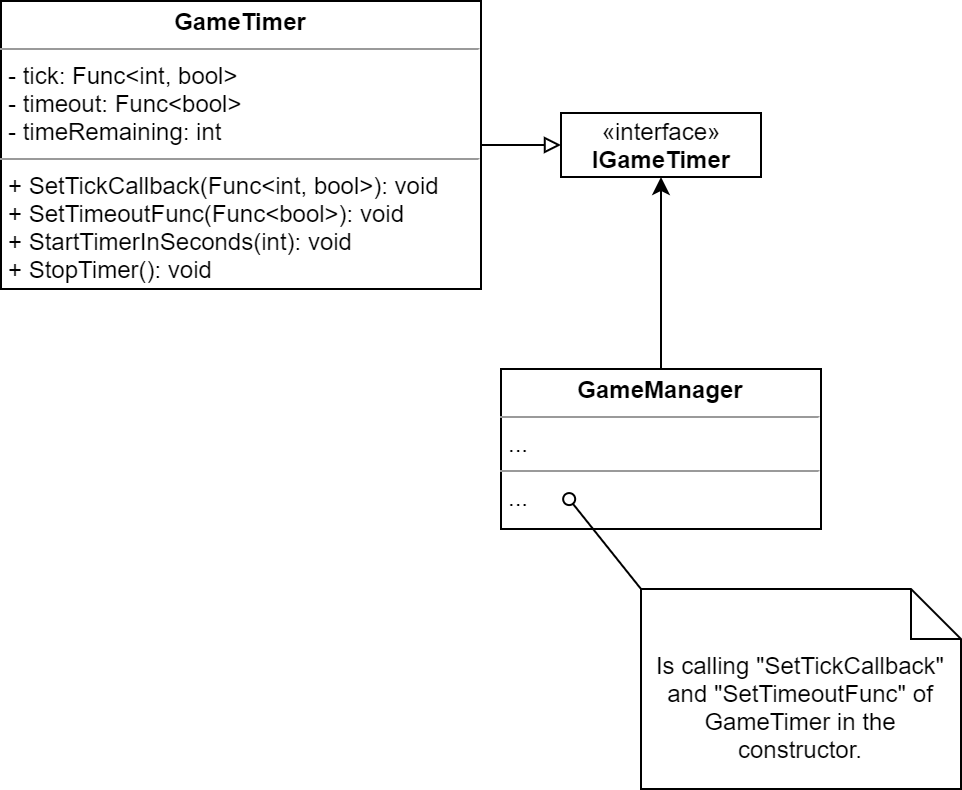
\includegraphics[width=0.7\textwidth]{Bilder/Entwurfsmuster.PNG}
\caption{\label{Abb:Entwurfsmuster}UML Diagramm des Beobachter Entwurfsmusters}
\end{figure}

\paragraph{Singleton}
Als zweites Entwurfsmuster wurde die Abwesenheit von Singletons festgestellt. Von jeder Klasse können mehrere Instanzen erzeugt werden und eine Klasse welche bei einem Aufruf wie \glqq GetInstance()\grqq{} die (einzige) Instanz einer anderen Klasse zurück gibt, gibt es nicht.

\endinput